\chapter{CASE STUDIES}

\onehalfspacing

\begin{enumerate}

\item \textbf{Rig Visit-RIG-IPS-M700}

\begin{itemize}

\item \underline{Location:} 

Sobahasan Field Cardwell 6

Rig Name-IPS M700-6

Rig Type-Mechanical Mobile

BOP Type-13 5/8 ” 5000 psi Double Ram and 5 5/8 ” 5000 psi Annular BOP

\vspace{1em}

\item \noindent{\underline{Mud Pump}}

Power-1250 hP

Power (in KW) - 700KWs

\vspace{1em}

\item \noindent{\underline{Well Details}}

Well Name-SBLR

Target Depth-1953.4 m

True Vertical Depth- 1920 m

Spud date- 29 th May’18

Well Profile-Inclined Well (Directional Drilling)

Kick Off Point-750 m

Net Horizontal Drift-138.98m

Angle-14.81 degrees

Azimuth- 24.1 degrees North

Pay Zone- 1441 m

\end{itemize}

%\begin{figure}[H]
%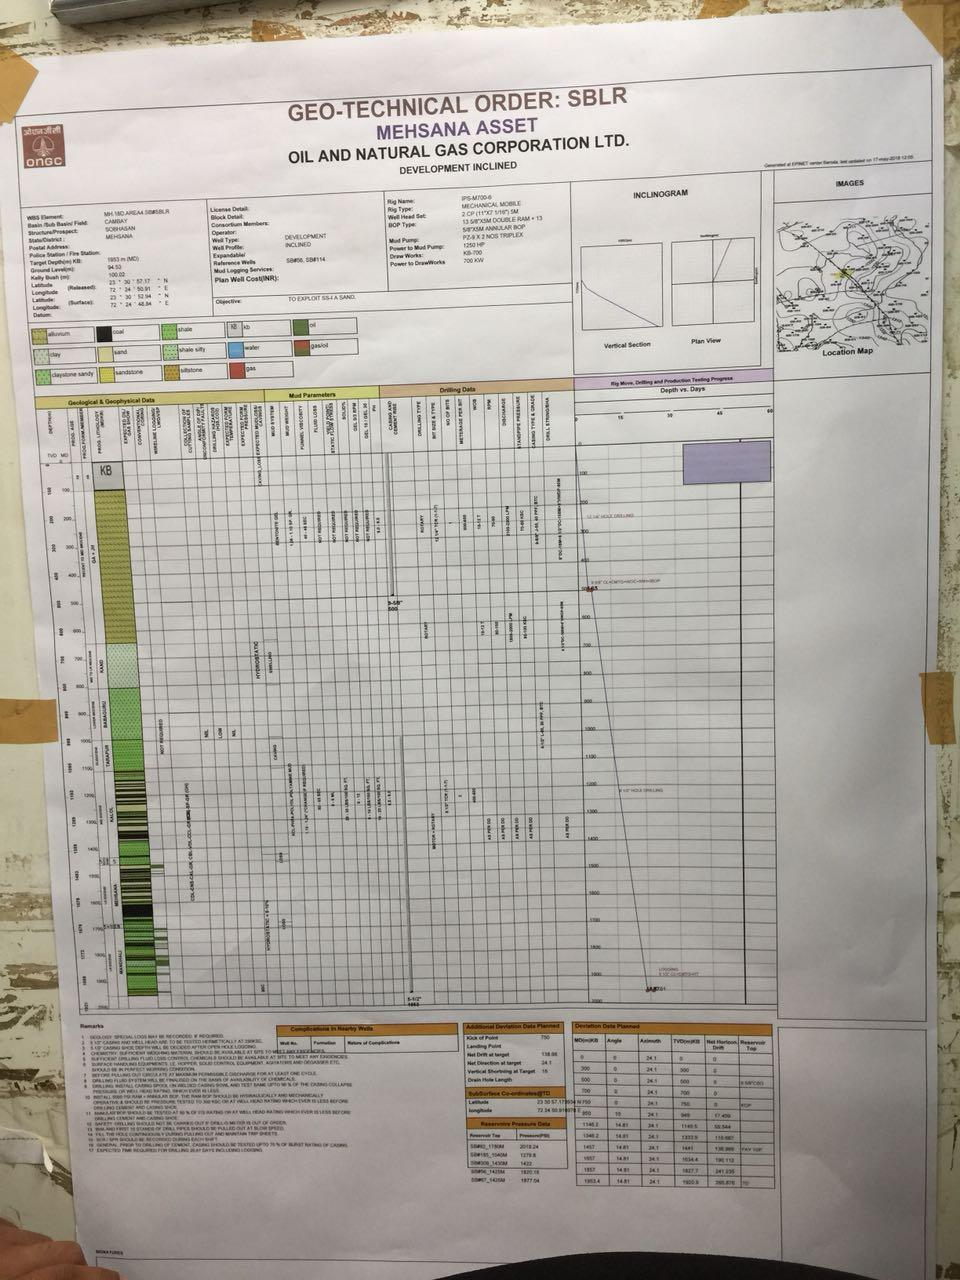
\includegraphics[scale=0.2]{images/GTO_IPS}
%\centering 
%\caption{A Picture of Geo Technical order of the Rig IPS-M700}
%\end{figure}

\noindent Observations at the Rig site are:

\begin{itemize}
\item Cementing Job was being done.
\item 500m depth was drilled.
\item Casing Policy- 2 CP (9 5/8 ” Conductor Casing and 5 1/2 ” Production Casing).
\item Specific Gravity of Cement- 1.83.
\item Class of Cement- Class G.
\item Thickening Time- 2- 3hours.
\end{itemize}

\begin{figure}[H]
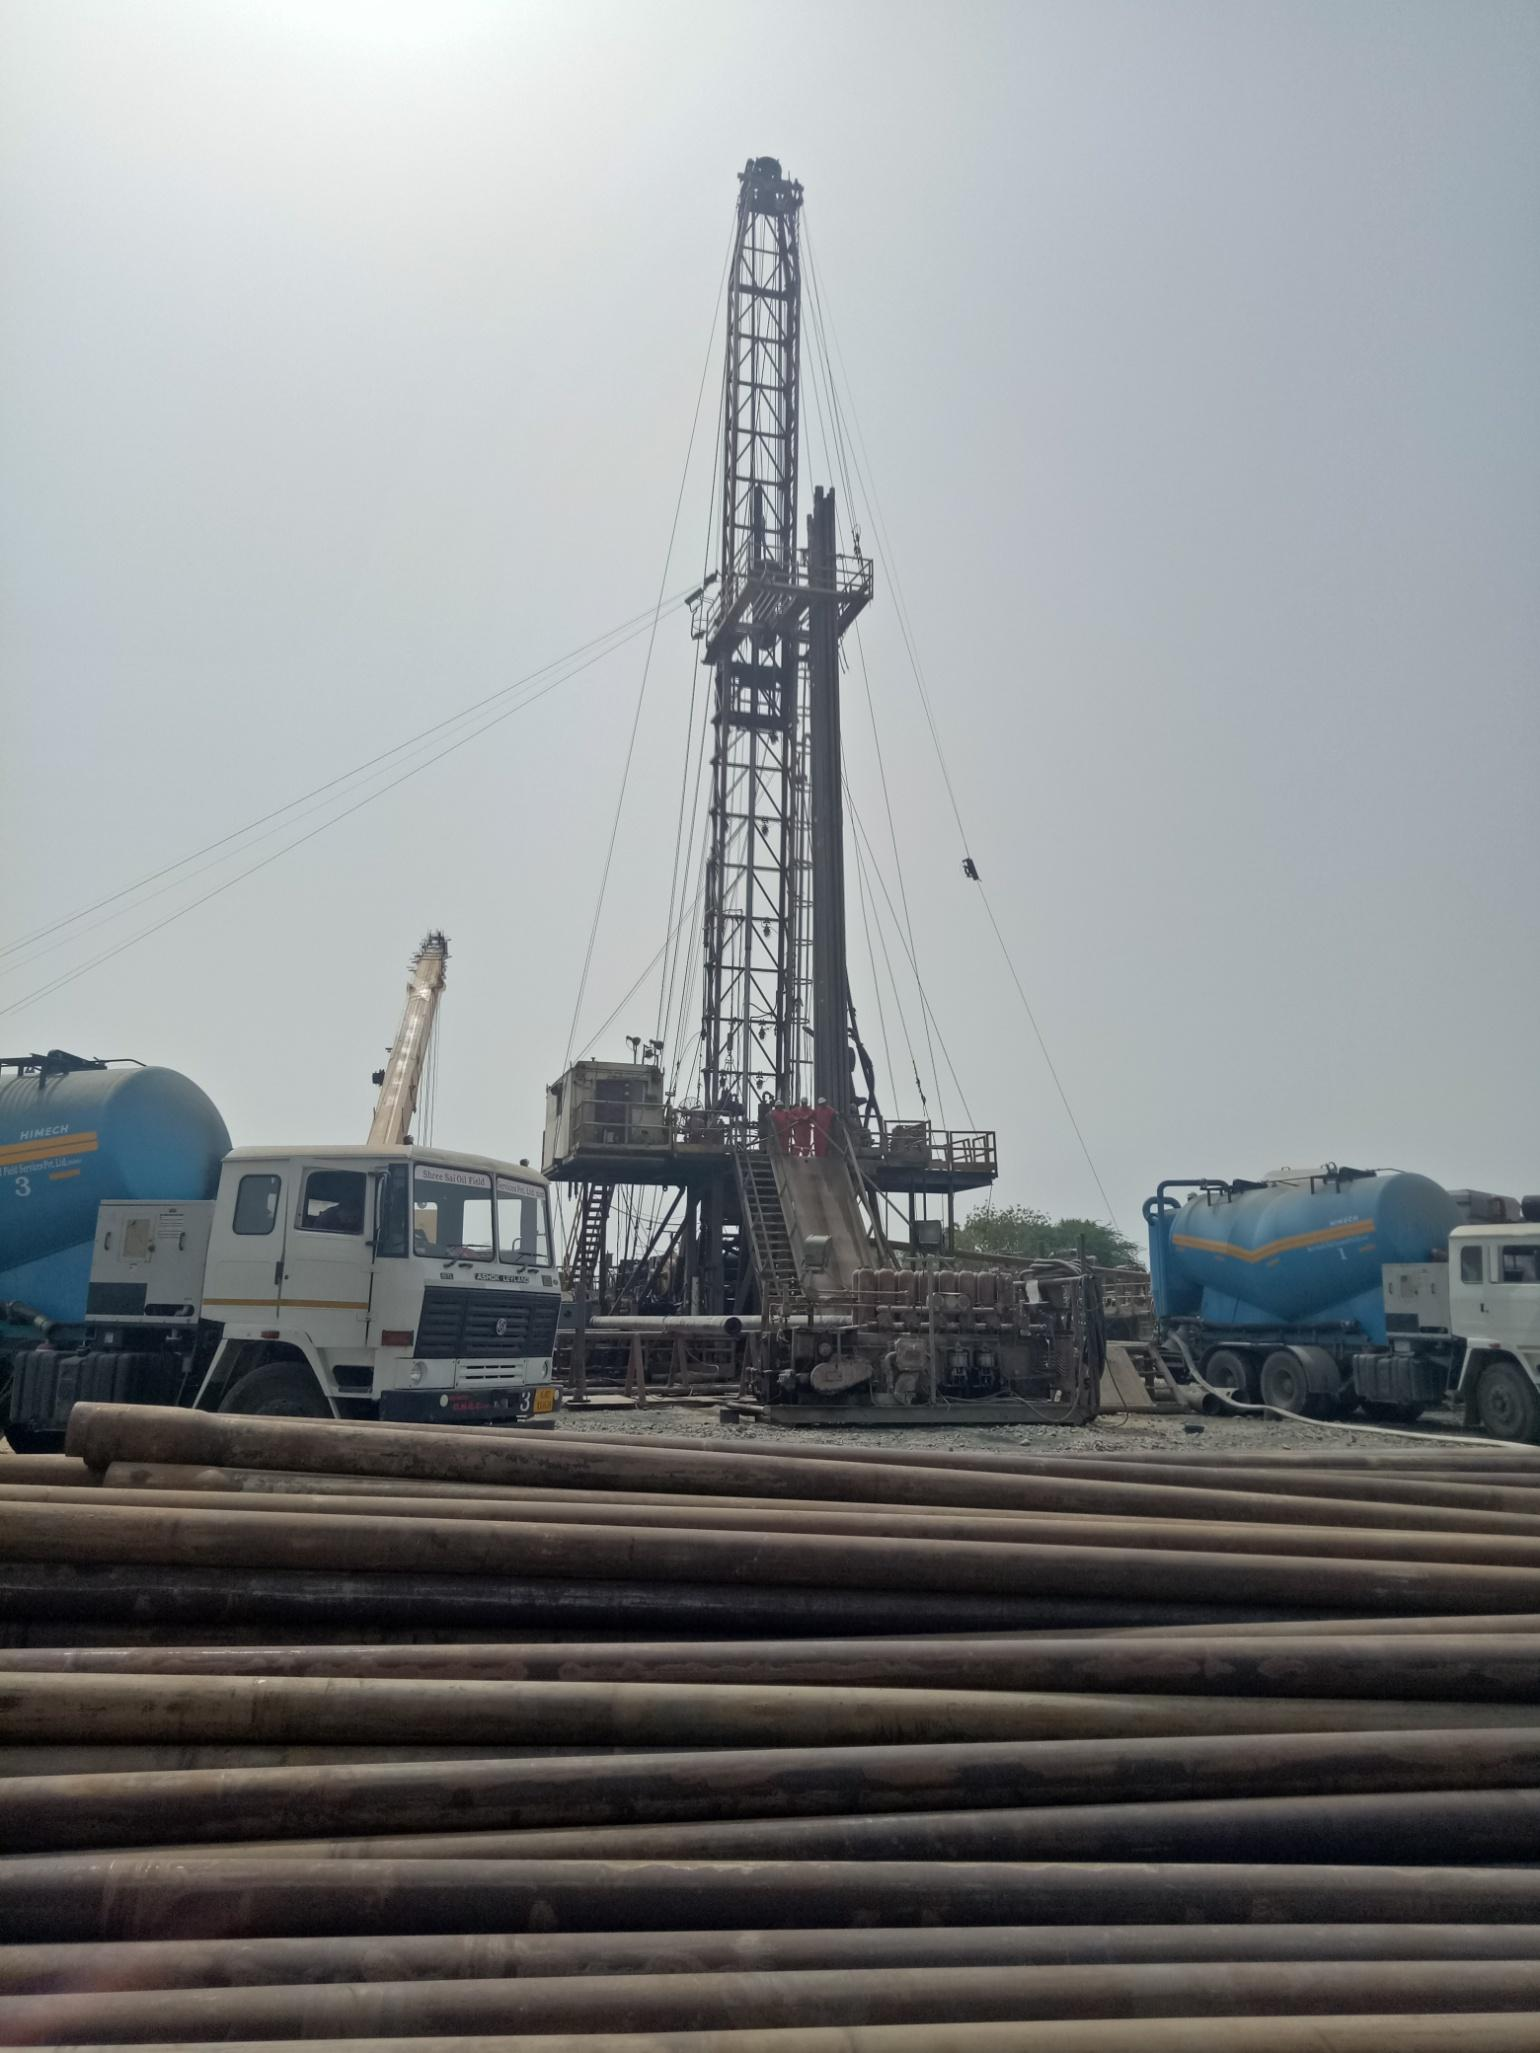
\includegraphics[scale=0.15]{images/IPS-M-700}
\centering 
\caption{A Picture of the Rig IPS-M700}
\end{figure}



\item \textbf{Rig E-760-18}

\vspace{1em}

\begin{itemize}

\item Location- Jotana
\item Rig Name- E-760-18

\item Rig Type- Electrical

\item BOP Rating- 13 3/8 ” 5000 psi double ram, 13 5/8 ” 5000 psi annular preventer

\item Mud Pump:Power-1000hp

\noindent Well Details:

\item Well Name- JNHL

\item Well Type- Development

\item Well Profile-Inclined

\item Target Depth-2204 m

\end{itemize}

\vspace{1em}

\noindent Well logging was being done and logging crew was taking the open
hole caliper log.

\begin{figure}[H]
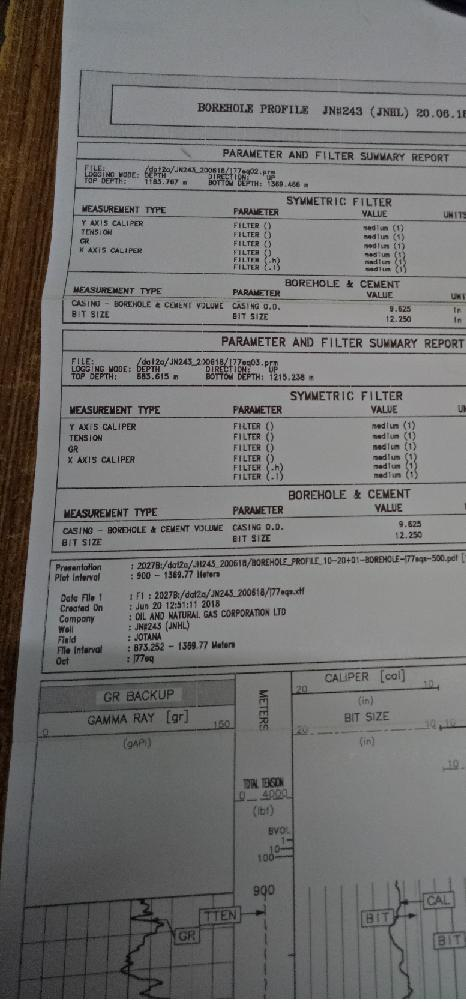
\includegraphics[scale=0.3]{images/Log}
\centering 
\caption{A Picture of the Caliper log}
\end{figure}

\textbf{Caliper Log:} A caliper log is a well logging tool that provides a
continuous measurement of the size and the shape of borehole along
its depth and is commonly used in hydrocarbon exploration and
development wells during drilling to keep a check on the hole size.

\vspace{1em}

The caliper tool measures the variation in the borehole diameter as it
is withdrawn from the bottom of the hole, using two or more
articulated arms that push against the bore hole wall. Each arm is
typically connected to a potentiometer which causes the resistance to
change as the diameter of the hole changes.



\end{enumerate}


 
